\documentclass[12pt,letterpaper]{article}
\usepackage{graphicx,textcomp}
\usepackage{natbib}
\usepackage{setspace}
\usepackage{fullpage}
\usepackage{color}
\usepackage[reqno]{amsmath}
\usepackage{amsthm}
\usepackage{fancyvrb}
\usepackage{amssymb,enumerate}
\usepackage[all]{xy}
\usepackage{endnotes}
\usepackage{lscape}
\newtheorem{com}{Comment}
\usepackage{float}
\usepackage{hyperref}
\newtheorem{lem} {Lemma}
\newtheorem{prop}{Proposition}
\newtheorem{thm}{Theorem}
\newtheorem{defn}{Definition}
\newtheorem{cor}{Corollary}
\newtheorem{obs}{Observation}
\usepackage[compact]{titlesec}
\usepackage{dcolumn}
\usepackage{tikz}
\usetikzlibrary{arrows}
\usepackage{multirow}
\usepackage{xcolor}
\newcolumntype{.}{D{.}{.}{-1}}
\newcolumntype{d}[1]{D{.}{.}{#1}}
\definecolor{light-gray}{gray}{0.65}
\usepackage{url}
\usepackage{listings}
\usepackage{color}

\definecolor{codegreen}{rgb}{0,0.6,0}
\definecolor{codegray}{rgb}{0.5,0.5,0.5}
\definecolor{codepurple}{rgb}{0.58,0,0.82}
\definecolor{backcolour}{rgb}{0.95,0.95,0.92}

\lstdefinestyle{mystyle}{
	backgroundcolor=\color{backcolour},   
	commentstyle=\color{codegreen},
	keywordstyle=\color{magenta},
	numberstyle=\tiny\color{codegray},
	stringstyle=\color{codepurple},
	basicstyle=\footnotesize,
	breakatwhitespace=false,         
	breaklines=true,                 
	captionpos=b,                    
	keepspaces=true,                 
	numbers=left,                    
	numbersep=5pt,                  
	showspaces=false,                
	showstringspaces=false,
	showtabs=false,                  
	tabsize=2
}
\lstset{style=mystyle}
\newcommand{\Sref}[1]{Section~\ref{#1}}
\newtheorem{hyp}{Hypothesis}

\title{Problem Set 2}
\date{October 23, 2025}
\author{Applied Stats/Quant Methods 1\\
	Shelly Veal-Upham\\
	25337422}

\begin{document}
	\maketitle

	\vspace{.5cm}
	\section*{Question 1: Political Science}
		\vspace{.25cm}
	The following table was created using the data from a study run in a major Latin American city.\footnote{Fried, Lagunes, and Venkataramani (2010). ``Corruption and Inequality at the Crossroad: A Multimethod Study of Bribery and Discrimination in Latin America. \textit{Latin American Research Review}. 45 (1): 76-97.} As part of the experimental treatment in the study, one employee of the research team was chosen to make illegal left turns across traffic to draw the attention of the police officers on shift. Two employee drivers were upper class, two were lower class drivers, and the identity of the driver was randomly assigned per encounter. The researchers were interested in whether officers were more or less likely to solicit a bribe from drivers depending on their class (officers use phrases like, ``We can solve this the easy way'' to draw a bribe). The table below shows the resulting data.\\

\begin{table}[h!]
	\centering
	\begin{tabular}{l | c c c }
		& Not Stopped & Bribe requested & Stopped/given warning \\
		\\[-1.8ex] 
		\hline \\[-1.8ex]
		Upper class & 14 & 6 & 7 \\
		Lower class & 7 & 7 & 1 \\
		\hline
	\end{tabular}
\end{table}

\begin{enumerate}
	
	\item [(a)]
	Calculate the $\chi^2$ test statistic by hand/manually (even better if you can do "by hand" in \texttt{R}).\\
\newpage

	First, I recreated the above table in R:\\
		\lstinputlisting[language=R, firstline=39, lastline=44]{PS02_SVU.R} 
	Then, created vectors of the expected values given formula \(f_{E}\frac{(Row\ Total)\times (Column\ Total)}{Grand\ Total}\) and used them to calculate the $\chi^2$ test statistic. To ensure this calculation is correct, I compared it to the $\chi^2$ test statistic from the \texttt{chisq.test()} in R-- both yield a value of \textbf{3.79}.\\
		\lstinputlisting[language=R, firstline=73, lastline=78]{PS02_SVU.R}  
		
	\item [(b)]
	Now calculate the p-value from the test statistic you just created (in \texttt{R}).  What do you conclude if $\alpha = 0.1$?\\
	\vspace{.1cm}
	
	Using \texttt{pchisq()} we can easily find that the p-value equals \textbf{0.1502}. At $\alpha = 0.1$, p$>\alpha$, meaning we cannot reject the null hypothesis and thus conclude that there may indeed be no statistical association between the two categorical variables (class and traffic stop outcome).\\
		\lstinputlisting[language=R, firstline=82, lastline=82]{PS02_SVU.R}  
		
	\item [(c)] Calculate the standardized residuals for each cell and put them in the table below.
	\vspace{.1cm}
	
	\begin{table}[h]
		\centering
		\begin{tabular}{l | c c c }
			& Not Stopped & Bribe requested & Stopped/given warning \\
			\\[-1.8ex] 
			\hline \\[-1.8ex]
			Upper class  & 0.136 & -0.815 & 0.819 \\
			\\
			Lower class & -0.183 & 1.094 & -1.099  \\
			
		\end{tabular}
	\end{table}
	\vspace{.1cm}
	
	I created this table by developing a numerator ("num") vector of observed - expected values and dividing by the square root of expected values, given formula  \(res=\frac{(f_{o}-f_{e})}{\sqrt{f_{e}}}\) and checked the results against the \texttt{chisq.test()} results.
		\lstinputlisting[language=R, firstline=108, lastline=109]{PS02_SVU.R}  
	
	\vspace{.1cm}
	\item [(d)] How might the standardized residuals help you interpret the results? \\
	\vspace{.1cm}
	
	Standardizing the residuals allows us to compare them to critical values (z-scores) on the standard normal distribution to see whether they show signficance in the association between the two variables. For a significance level of  $\alpha = 0.1$ the critical value of z in a two-tailed test is $z = \pm 1.645$. None of (the absolute value of) our standardized residuals are above 1.645, signaling a lack of signficance in association between the two categorical variables.\\
	
\end{enumerate}

\newpage

\section*{Question 2: Economics}
Chattopadhyay and Duflo were interested in whether women promote different policies than men.\footnote{Chattopadhyay and Duflo. (2004). ``Women as Policy Makers: Evidence from a Randomized Policy Experiment in India. \textit{Econometrica}. 72 (5), 1409-1443.} Answering this question with observational data is pretty difficult due to potential confounding problems (e.g. the districts that choose female politicians are likely to systematically differ in other aspects too). Hence, they exploit a randomized policy experiment in India, where since the mid-1990s, $\frac{1}{3}$ of village council heads have been randomly reserved for women. A subset of the data from West Bengal can be found at the following link: \url{https://raw.githubusercontent.com/kosukeimai/qss/master/PREDICTION/women.csv}\\

\noindent Each observation in the data set represents a village and there are two villages associated with one GP (i.e. a level of government is called "GP"). Figure~\ref{fig:women_desc} below shows the names and descriptions of the variables in the dataset. The authors hypothesize that female politicians are more likely to support policies female voters want. Researchers found that more women complain about the quality of drinking water than men. You need to estimate the effect of the reservation policy on the number of new or repaired drinking water facilities in the villages.
\vspace{.1cm}
\begin{figure}[h!]
	\caption{\footnotesize{Names and description of variables from Chattopadhyay and Duflo (2004).}}
	\vspace{.5cm}
	\centering
	\label{fig:women_desc}
	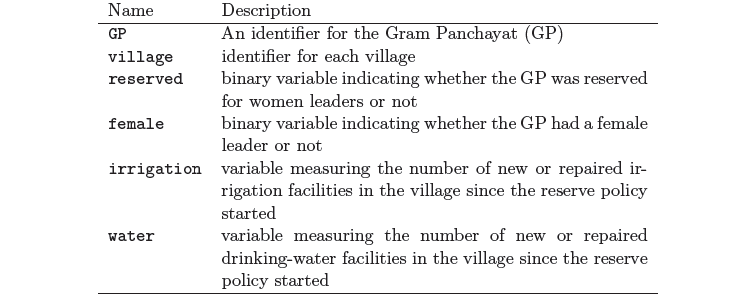
\includegraphics[width=1.1\textwidth]{women_desc.png}
\end{figure}		

\newpage
\begin{enumerate}
	\item [(a)] State a null and alternative (two-tailed) hypothesis. \\
	\vspace{.2cm}
	
	\textbf{Null:} On average, there is no difference in the number of new or repaired drinking water facilities between villages with and without the reservation policy (that is, $\beta_{1} = 0$). \\
	\textbf{Alternative:} There is an average difference in the number of new or repaired drinking water facilities between villages with and without the reservation policy ($\beta_{1} \neq 0$).\\
	
	\vspace{.1cm}
	\item [(b)] Run a bivariate regression to test this hypothesis in \texttt{R} (include your code!).\\
	\vspace{.2cm}
	
	Running the following code results in line $y = \beta_{0} + \beta_{1}*x$ with $\beta_{0} = 14.74$, $\beta_{1} = 9.25$, $R^2 = 0.0169$, and a p-value for $\beta_{1}$ of 0.0197 (plus, a plot for visualizing).
		\lstinputlisting[language=R, firstline=137, lastline=143]{PS02_SVU.R}  
		
	\vspace{.1cm}
	\item [(c)] Interpret the coefficient estimate for reservation policy. \\
	\vspace{.2cm}
	
	Our estimated water drinking facilities (based on binary input variable of 0/1 for F/T regarding the use of the reservation policy) is modeled by $y = 14.74 + 9.25*x$. The intercept, 14.74 suggests that on average there were 14-15 new (or repaired) drinking water facilities in villages that did not reserve seats on the GP for women. This is in comparison to 23.99, or 24, the estimated number of new (or repaired) drinking water facilities in villages with GP seats reserved for women. \\
	
	The significance of this difference is signaled by the p-value of $\beta_{1}$ being 0.0197 (less than $\alpha = 0.05$). This means we can reject the null hypothesis that there is no average difference in the number of new or repaired drinking water facilities between villages with and without the reservation policy.\\
	
	Still, it is notable that the $R^2$ value is rather small, suggesting that the model itself accounts for only 1.7\% of variation in the dataset.\\

\end{enumerate}

\end{document}
